% Filename  : samplepaper.tex
% Purpose   : A sample exam paper to demonstrate how to use the 'ditpaper'
%             TeX class.
% Author    : Emmet Caulfield
% Revision  : $Id: samplepaper.tex 2 2006-02-19 20:34:45Z emmet $
% Repository: $HeadURL: http://svn.netrogen.lan/tex-ditpaper/trunk/samplepaper.tex $
%

% 'nosolution' (default) and 'solution' toggle the inclusion of solutions
% in the output. The tag nosolution, below, is replaced by 'sed' 
% in the Makefile to cause both the paper and the solutions to be produced.
\documentclass[nosolution]{ditpaper}

\usepackage{graphicx}
\usepackage{multirow}
\usepackage{rotating}


% These must be set or bizarre defaults will be used:
\facility{Kevin Street, Dublin 8}
\course{BSc. (Hons) in Computer Science}
\examcode{RS249/401C}
\stage{Stage 4}
\session{Supplemental Examinations 2012}
\title{Artificial Intelligence II}
\examiners{Dr. John Kelleher\\
Dr. Deirdre. Lillis\\
Mr. Ray Walshe}
\examdate{}
\examtime{Duration: 2 Hours}
\instructions{Question 1 is \textbf{compulsory}\par{} Answer Question 1 (40 marks) \textbf{and}\par{} any 2 Other Questions (30 marks each).}


\begin{document}


%aima chapters 18
% inductive bias, learning theory - supervised/unsupervised, overfitting, lazy/eager learner, classification v regression, false positive v false negatives, linear separability, consistency, evaluation

\question
\begin{enumerate}
	\item Explain what is meant by \textbf{inductive learning}.
	\marks{5}
	\begin{answer}
		Inductive Learning involves the process of learning by example � where a system tries to induce a general rule from a set of observed instances
	\end{answer}
	\item Explain what can go wrong when a machine learning classification algorithm uses the wrong inductive bias.
		\marks{5}
		\begin{answer}
			\begin{itemize}
				\item If the inductive bias of the learning algorithm constrains the search to only consider simple hypotheses we may have excluded the real function from the hypothesis space. In other words, the true function is \textbf{unrealizable} in the chosen hypothesis space, (i.e., we are \textbf{underfitting}). 
				\item If the inductive bias of the learning algorithm allows the search to consider complex hypotheses, the model may hone in on irrelevant factors in the training set. In other words the model with \textbf{overfit} the training data.
			\end{itemize}
\end{answer}
	\item  Inductive machine learning is often referred to as an \textbf{ill-posed problem}. What is meant by this description?
	\marks{10}
	\begin{answer}
		Inductive machine learning algorithms essentially search through a hypothesis space to find a the best hypothesis that is consistent with the training data used. It is possible to find multiple hypotheses that are  consistent with a given training set (i.e. agrees with all training examples).  It is for this reason that inductive machine learning is referred to as an ill-posed problem as there is typically not enough information in the training data used to build a model to choose a single best hypothesis. Inductive machine learning algorithms must somehow choose one of the available hypotheses as the \emph{best}. An example like that shown in the figure below would be useful at this point
		\begin{center}
			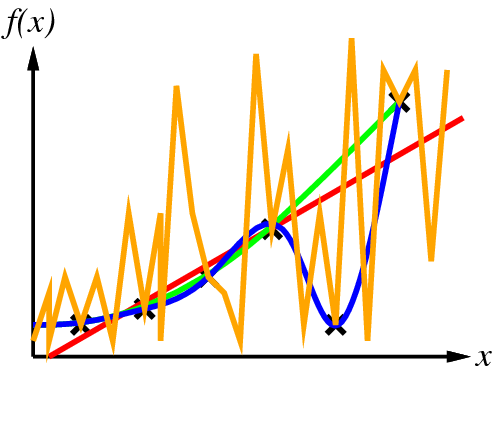
\includegraphics[width=5cm]{./images/curve-fitting5.png}
		\end{center}
	\end{answer}
	\item Let us say we have three classification algorithms. How can we order these three from best to worst?
	\marks{20}
	\begin{answer}
		This is a discursive question so giving a precise answer is not appropriate. However, key points that the student should touch on include:
		\begin{itemize}
		\item Predictive accuracy
		\item Speed and scalability 
		\begin{itemize}
			\item Time to construct the model
			\item Time to use the model
		\end{itemize}
		\item Robustness (handling noise and missing values)
		\item Scalability
		\item Interpretability (understanding and insight provided by the model)
	\end{itemize}
	It should be noted also, that these evaluation criteria are application dependent.
	\end{answer}
\end{enumerate}


\newpage

%Q2
% knn and CBR 
% information theory, entropy, Decision Trees, Inductive logic programming
		
			
\question 
	\begin{enumerate}
			\item Discuss the advantages and disadvantages of \textbf{$k$-Nearest Neighbour} classification.
				\marks{5}
				\begin{answer}
				Strengths
				\begin{enumerate}	
					\item No training involved  lazy learning
					\item New data can be added on the fly
					\item Some explanation capabilities
					\item Robust to noisy data by averaging k-nearest neighbors
				\end{enumerate}
				Weaknesses
				\begin{enumerate}
					\item Not the most powerful classification (generally its accuracy will be lower than an ANN or SVM model)
					\item Slow classification 
					\item Curse of dimensionality (as you increase the number of features you need more and more examples to cover the problem space - kNN are particularly susceptible to this issue as they do not do any feature selection).
				\end{enumerate}
			\end{answer}
			
		\item IT-Tunes is on online music sales service that is trying to build an inductive machine learning system to recommend new songs to its users. They have collected a dataset that records details of songs they sell and details of ratings that users have given these songs (missing values in the ratings columns indicate that a user has not rated a particular song). The table below shows an extract from this dataset showing details of $5$ songs and associated ratings for $5$ users (note that in the full dataset there are many more songs and many more users).

			\begin{small}
			\begin{center}
			\begin{tabular}{|r|c|c|c|c|c|}
			\hline
			\textbf{ID} 				& 001 		& 004			& 007 	& 011 		& 022\\
			\hline	
			\textbf{Title} 			& Jeremy 		& One 			& Please 	& Fool's Game 	& Help!\\
			\textbf{Album} 			& Ten 		& Achtung Baby	& Pop 	& M. Bolton 	& Help!\\
			\textbf{Artist} 			& Pearl Jam 	& U2 			& U2 	& M. Bolton 	& The Beatles\\
			\textbf{Year} 			& 1990 		& 1992 			& 1997 	& 1983 		& 1965\\
			\textbf{Genre} 			& Rock 		& Rock 			& Rock 	& Soul 		& Pop\\
			\textbf{Best Chart Pos} 	& 10 			& 1 				& 6 		& 25 			& 1\\
			\hline
			\textbf{User1-Score} 		& 3 			& 2				& 2		& 5			& 4\\
			\textbf{User2-Score} 		& 5 			& -				& 5		& -			& 4\\
			\textbf{User3-Score} 		& 5 			& 2				& 2		& 1			& 1\\
			\textbf{User4-Score} 		& 1 			& -				& -		& -			& 1\\
			\textbf{User5-Score} 		& - 			& 1				& 1		& 5			& 3\\
			\hline
			\end{tabular}
			\label{tab:songs}
			\end{center}
			\end{small}

		\begin{enumerate}
			\item In order to build a case based reasoning (CBR) classification system to predict whether a user would like a particular song, or not, a case representation is required. Describe a case structure for the dataset shown in the table above that could be used to build a CBR system that would predict the rating a particular user would be likely to give to a particular song. Justify any decisions that you make and explain any assumptions used.
			\marks{5}
			\begin{answer}
			Any reasonable system will be acceptable here as long as it is justified. Issues that should be addressed include:
				\begin{enumerate}
				\item Which features actually hold information that is likely to relate to the problem?
				\item Can a balance be struck between internal features (such as song titles, years etc) and external features (such as user ratings)
				\item Can derived features by created from the features present in the dataset?
				\end{enumerate}
			\end{answer}
			\item A good similarity measure is crucial for any CBR system. Describe a similarity measure that would be appropriate for comparing cases in the structure described in the answer part (i) of this question. Justify any decisions that you make and explain any assumptions used.
			\marks{5}
			\begin{answer}
				Again any reasonable answer will be accepted here. Issues that should be addressed include:
				\begin{enumerate}
				\item Normalisation
				\item How can various elements within a hybrid similarity measure be combined in order to make a complete similarity measure?
				\item How can the various elements present in the feature set be compared?
				\end{enumerate}
			\end{answer}
			\item Is \textbf{case-based reasoning} the most appropriate inductive machine learning technique to use for this prediction problem?
				\marks{5}
				\begin{answer}
								Again students have a fairly free hand in answering this question. Issues that should be addressed include:
								\begin{itemize}
									\item The ability to add new instances when new information becomes available.
									\item the need to build classification models for each customer
									\item Is a classification model the best approach, or would something like collaborative filtering be more appropriate?
								\end{itemize}
				\end{answer}
		\end{enumerate}

		% Information theory and Decision Trees
		\item In the context of Decision Tree Learning define what is meant by the following terms:
			\begin{enumerate}
			%Callan
					\item entropy
					\marks{5}					
					\begin{answer}
				For $c$ classification categories the entropy $E$ is defined as: $E=\sum_{i=1}^{c} -p_i\ log_2\ p_i$ where $p_i$ is the probability of category $i$ occurring.
					\end{answer}
			%Callan
			\item information gain
					\marks{5}
			\begin{answer}
				The information gain for an attribute is the expected reduction in entropy if the examples were to be partitioned according to that attribute and is defined as: $Gain(T,A)=E(T) - \sum_{j=1}^{v} \frac{|T_{j}|}{|T|}E(T_{j})$ where $T$ is a set of training examples and $T_j$ is a subset of examples having value $j$ for attribute $A$ 
			\end{answer}
			\end{enumerate}
	\end{enumerate}

\newpage
	
%Q3 30 marks
% basic probability 5
% bayesian networks 10
% bayesian learning  15

\begin{table}[htb]
\caption{Full joint probability distribution for a dentist visit}
\begin{center}
\begin{tabular}{c|c|c|c|c|}
                          & \multicolumn{2}{c}{$toothache$} \vline & \multicolumn{2}{c}{$\lnot toothache$}  \vline \\
\hline
                          & $catch$ & $\lnot catch$ & $catch$ & $\lnot catch$ \\
 $cavity$          & 0.108     & 0.012             & 0.072      & 0.008             \\
 $\lnot cavity$ & 0.016     & 0.064             & 0.144      & 0.576             \\
\end{tabular}
\end{center}
\label{tab:fjd}
\end{table}%

\begin{figure}
		\begin{center}
	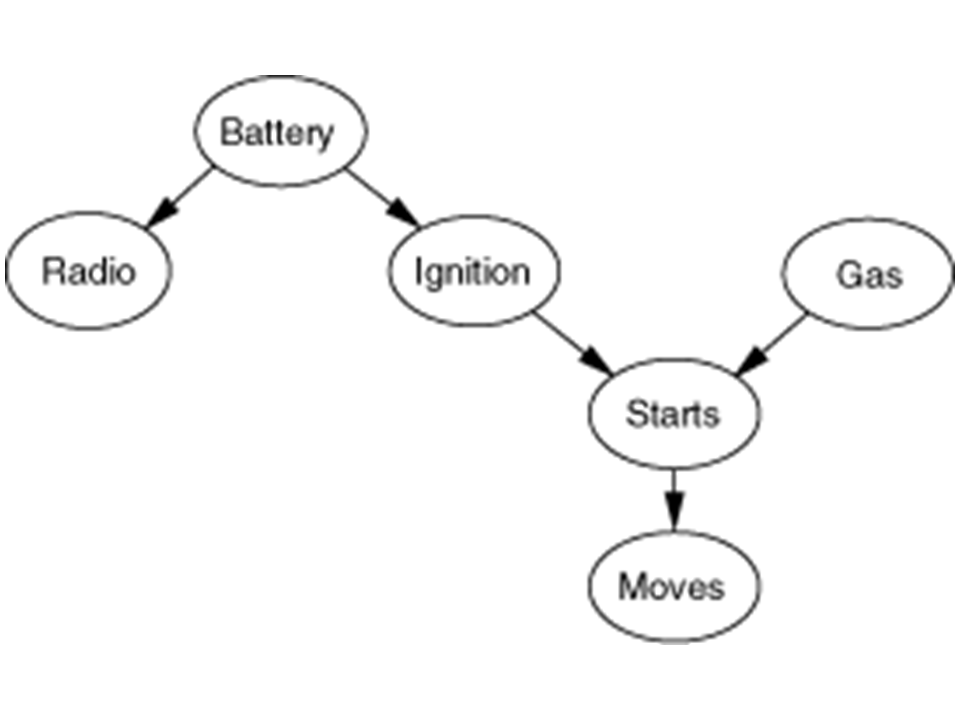
\includegraphics[width=2.5in]{./images/car-starts.png}
		\end{center}
	\caption{A Bayesian network of a car's electrical system and engine. Each variable is boolean and the true value indicates that the corresponding aspect of the vehicle is in working order.}
	\label{fig:carsystem}
\end{figure}

\question
	\begin{enumerate}
		%basic probability
		\item Given the full joint distribution shown in Table \ref{tab:fjd}, calculate:
				\begin{center}
				 	$\textbf{P}(Cavity|toothache \lor catch)$
				\end{center}
				\marks{5}
				\begin{answer}
					This asks for the vector of probability values for $Cavity$, given that either $Toothache$ or $Catch$ is true.\\
					Recall $P(a|b) = \frac{P(a \land b)}{P(b)} \rightarrow$ \\
					$\textbf{P}(Cavity|toothache \lor catch) =$\\
					 $\langle \frac{P(cavity \land (toothache \lor cavity))}{P(toothache \lor catch)}, \frac{P(\lnot cavity \land (toothache \lor cavity))}{P(toothache \lor catch)}\rangle$\\
					First compute $P(toothache \lor catch) = 0.108 + 0.012 + 0.016 + 0.064 + 0.072 + 0.144 = 0.416$. \\
					Then $\textbf{P}(Cavity | toothache \lor catch ) =$\\
					 $\langle \frac{0.108 + 0.012 + 0.072}{0.416}, \frac{0.016 + 0.064 + 0.144}{0.416}\rangle = \langle 0.4615, 0.5384\rangle$ \\
				\end{answer}
		%bayesian networks

		\item  Consider the network for car diagnosis shown in Figure \ref{fig:carsystem}.
		\begin{enumerate}
			\item Extend the network with the Boolean variables \textit{IcyWeather} and \textit{StarterMotor}; assume that a \textit{StarterMotor} effects whether or not the car \textit{Starts} and that \textit{Icy Weather} effects the \textit{Battery} and the \textit{StarterMotor}, 
			\marks{5}
			\begin{answer}
			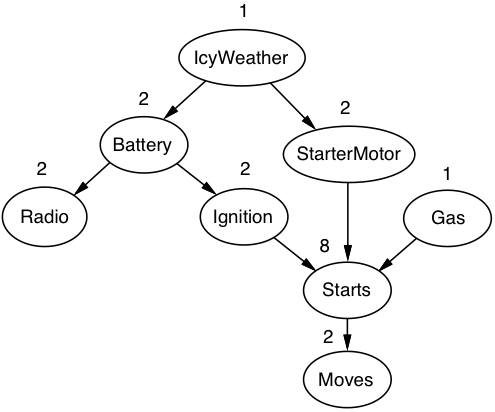
\includegraphics[width=2.5in]{./images/car-extended.png}
			\end{answer}
			\item How many independent values are contained in the full joint probability distribution?
			\marks{5}
			\begin{answer}
			With 8 Boolean variables, the joint has $2^{8}?1 = 255$ independent entries. 
			\end{answer}
		\end{enumerate}		
		%bayesian learning
		\item You are on holidays on Fisher Island. The yearly weather on Fisher Island comes in five different varieties: 
			\begin{itemize}
				\item there is a 10\% chance that there will be rain everyday of the year.
				\item there is a 20\% chance that there will be rain on 75\% of the days of the year.
				\item there is a 40\% chance that there will be rain on 50\% of the days of the year.
		    		 \item there is a 20\% chance that there will be rain on 25\% of the days of the year.
		     		\item there is a 10\% chance that there will be no rain on any day of the year.
			\end{itemize}
			\begin{enumerate}
				\item Given that it has rained on day 1 and 2 of the year compute the posterior probability of each of the 5 yearly weather patterns on day 2 of the year. Give your answer rounded to four places of precision.
				\marks{10}
				\begin{answer}
						To begin we will define some notation. Let: 
						\begin{itemize}
							   \item $h_1$ denote the hypothesis that it will rain everyday, $P(h_1)=0.1$.
					\item $h_2$ denote the hypothesis that it will rain on 75\% of the days of the year, with prior $P(h_2)=0.2$.
					\item $h_3$ denote the hypothesis that it will rain on 50\% of the days of the year, with prior $P(h_3)=0.4$.
					\item $h_4$ denote the hypothesis that it will rain on 25\% of the days of the year, with prior $P(h_4)=0.2$.
					\item $h_5$ denote the hypothesis that there will be no rain during the year, with prior $P(h_5)=0.1$.
					\end{itemize}
					Also, if we use the notation $rain_x$ to represent the observation of rain on day x of the year, then the probability of rain on a day of the year given a particular hypothesis $h$ is:
					\begin{itemize}
						\item $P(rain_x|h_1)=1.0$ .
						\item $P(rain_x|h_2)=0.75$ .
						\item $P(rain_x|h_3)=0.5$ .
						\item $P(rain_x|h_4)=0.25$ .
						\item $P(rain_x|h_5)=0.0$ .
					\end{itemize}
					Then:
						\begin{itemize}
							\item By Bayes' rule, we can compute the posterior probability of a hypothesis given the data so far using: $P(h_i|\textbf{d}) = \alpha P(\textbf{d}|h_i) P(h_i)$
				      		\item And, the likelihood of the data given a hypothesis is calculated using: $P(\textbf{d}|h_i) = \prod_j P(d_j|h_i)$
				           \end{itemize}
				       So:
				\begin{itemize}
					\item $P(h_1|rain_1,rain_2)=\alpha (\prod_{j=1}^2 P(rain_j|h_1))P(h_1)=\alpha 1.00^2 \times 0.1=\alpha 0.1=\frac{0.1}{0.325} \approx .3077$.
					\item $P(h_2|rain_1,rain_2)=\alpha (\prod_{j=1}^2 P(rain_j|h_2))P(h_1)=\alpha 0.75^2 \times 0.2=\alpha 0.1125=\frac{0.1125}{0.325} \approx .3461$.
					\item $P(h_3|rain_1,rain_2)=\alpha (\prod_{j=1}^2 P(rain_j|h_3))P(h_1)=\alpha 0.50^2 \times 0.4=\alpha 0.1=\frac{0.1}{0.325} \approx .3077$.
					\item $P(h_4|rain_1,rain_2)=\alpha (\prod_{j=1}^2 P(rain_j|h_4))P(h_1)=\alpha 0.25^2 \times 0.2=\alpha 0.0125=\frac{0.0125}{0.325} \approx .0385$.
					\item $P(h_5|rain_1,rain_2)=\alpha (\prod_{j=1}^2 P(rain_j|h_5))P(h_1)=\alpha 0.00^2 \times 0.1=\alpha 0.0=0.0$.
				\end{itemize}
			\end{answer}
			\item Given that after the first 10 days of the year the weather has been such that the posterior probabilities of each of the 5 varieties of the yearly weather on Fisher Island are:  
					\begin{itemize}
						\item there is now a 90\% chance that there will be rain everyday for the rest of the year; 
						\item a 7\% chance that there will be rain on 75\% of the rest of the days of the year;  
						\item a 2\% chance that there will be rain on 50\% of the rest of the days of the year; 
						\item a 1\% chance that there will be rain on 25\% of the rest of the days of the year; 
						\item and there is a 0\% chance that there will be no rain for the rest of the year. 
					\end{itemize}
					What is the Maximum a Posterior (MAP) probability of rain on day 11?
							   \marks{5}
				         \begin{answer}
				         A MAP prediction just uses the prediction provided by the single most probable hypothesis. In this instance the single most probable hypothesis is the hypothesis that it will rain on every day of the year. This hypothesis would predict rain on day 11 with probability of 1.0 (i.e. certainty)
				         \end{answer}
		\end{enumerate}
	\end{enumerate} %end Q3

%
\newpage

%Q4
%Linear Regression Neural Nets, SVMs, Ensemble Learning
\begin{table}
\begin{center}
\begin{tabular}{cccccc}
\hline
x & 0 & 1 & 2 & 3 & 4\\
\hline
y & 3 & 6 & 7 & 8 & 11\\
\hline
\end{tabular}
\caption{Example Dataset for Linear Regression Question}
\label{tab:linregTab2}
\end{center}
\end{table}

\question 
	\begin{enumerate}
		%Regression Learning		
\item Assuming a domain with one explanatory variable $x$ and one dependent variable $y$ linear regression uses the following formula to model the relationship between the explanatory and dependent variable: 
	\begin{center}
		$f(x) = w_1x + w0$
	\end{center}
where $w1$ and $w0$ are computed using the following formulae (where $M$ is number of data points in the dataset):
	\begin{large}
	\begin{center}
		$w_1 =  \frac{(M \sum_{i=1}^M x_i y_i) - (\sum_{i=1}^{M} x_i \sum_{i=1}^{M} y_i)} {(M \sum_{i=1}^{M} x_i^2) - (\sum_{i=1}^{M} x_i)^2}$
	\end{center}
	\begin{center}
		$w_0 = (\frac{1}{M} \sum_{i=1}^{M} y_i) - (\frac{w_1}{M} \sum_{i=1}^{M} x_i)$
	\end{center}
	\end{large}
Using the data in Table \ref{tab:linregTab2} compute the values of $w_0$ and $w_1$ that provide the best linear fit to the data.
			\marks{10}
			\begin{answer}
				First we need to compute the values of the equation components:
			\begin{itemize}
				\item M = 5
				\item $\sum_{i=1}^{M} x_i y_i = 0 + 6 + 14 + 24 + 44 = 88$
				\item $\sum_{i=1}^{M} x_i = 10$
			   	\item $\sum_{i=1}^{M} y_i = 35$
			  	\item $\sum_{i=1}^{M} x_i^2 = 0 + 1 + 4 + 9 + 16 = 30$
			  	\item $(\sum_{i=1}^{M} x_i)^2 = 10^2 = 100$
			\end{itemize}
				Given these values,  $w_1$:
				\begin{center}
					\textbf{$w_1= \frac{(5*88)-(10*35)}{(5*30)-100} = \frac{90}{50}=1.8$}
				\end{center}
				And, $w_0$:
				\begin{center}
				\textbf{$w_0= (\frac{1}{5}*35) - (\frac{1.8}{5}*10)= 7-3.6=3.4$}
			\end{center}
			\end{answer}
		%Neural Nets	
		\item What does it mean if two classes $C_1$ and $C_2$ are described as \textbf{linearly separable}?
			\marks{5}
		\begin{answer}
			This means that for each class $C_i$ there exists a hyperplane $H_i$ such that on its positive side lie all $x \in C_i$ and on its negative side lie all $x \in C_j , j \ne i$
		\end{answer}
 		\item Describe the processing stages of a McCulloch-Pits ''unit''.
			\marks{7}
		\begin{answer}
			The processing stages of a unit are:
			\begin{enumerate}
			\item Each unit $i$ first compute a weighted sum of its inputs:  $in_i \leftarrow \sum_j W_{j,i}  a_j$
			\item Then it applies an \textbf{activation function} $g$ to this sum to derive the output (activation) $a_i$: $a_i \leftarrow g(in_i) = g\left(\sum_j W_{j,i} a_j\right)$
			\end{enumerate}
			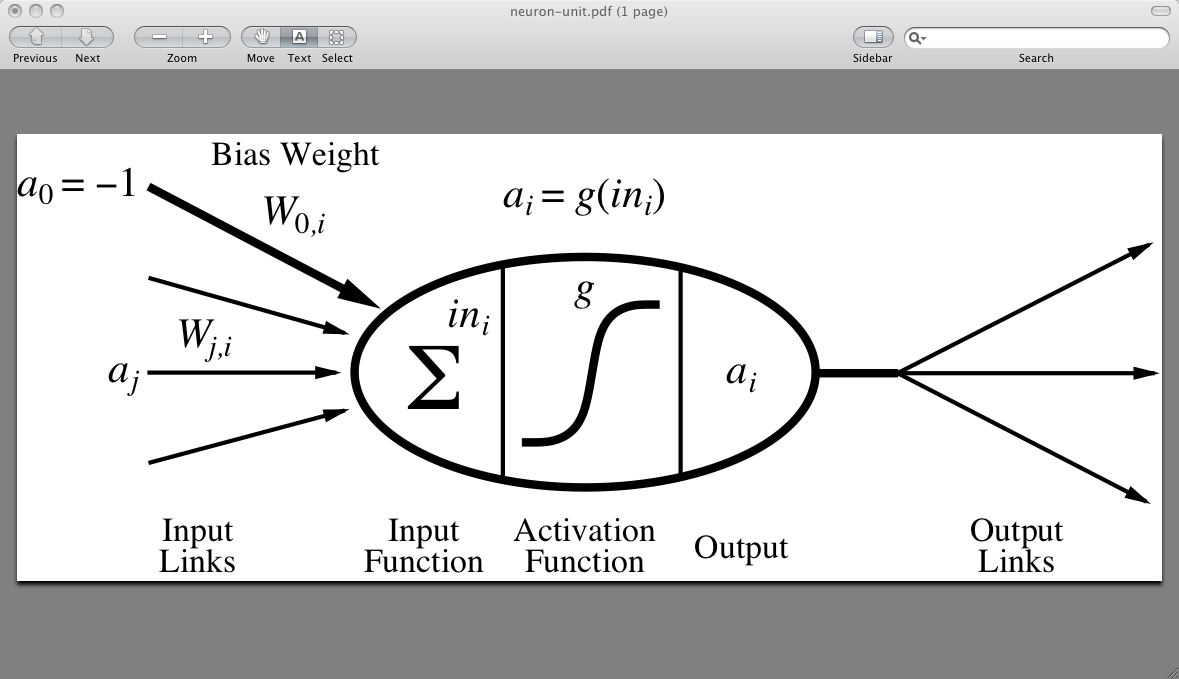
\includegraphics[width=3.5in]{./images/neuron-unit.png}
		\end{answer}
\question Figure \ref{fig:mystery-perceptron} is a schematic of a 3 input perceptron. Input $a_0$ is fixed at $a_0 = -1$, inputs $a_1$ and $a_2$ are binary. The perceptron uses a threshold activation function that outputs a 1 if the weighted sum of inputs is greater than 0 and a 0 otherwise. Define the \textbf{truth-table of the function} that this perceptron implements \emph{and} identify the \textbf{name of the function}. 
		\marks{8}
		\begin{answer}
		   {\Large
   \begin{tabular}{@{} ccc | c | c @{}}
      \multicolumn{3}{c}{Inputs} & $in_i$ & $a_i$ \\ \hline
      $a_0$ & $a_1$ & $a_2$ & $\sum_{j=0}^{2} w{j}{i} a_j$ & $\left( in_i  > 0\right)?(1):(0)$\\ \hline
      -1 & 1 & 1 & 0.5 & 1\\
      -1 & 1 & 0 & -0.5 & 0\\
      -1 & 0 & 1 & -0.5 & 0\\
      -1 & 0 & 0 & -1.5 & 0\\ \hline        
   \end{tabular}
   }\\
This perceptron implements the AND function.
		\end{answer}
	\end{enumerate}

\begin{figure}[h]
	\begin{center}
 		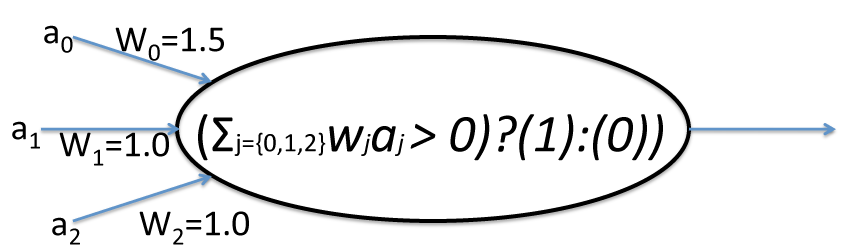
\includegraphics[width=4in]{./images/mystery-perceptron.png}
	\end{center}
		\caption{A 3 input perceptron. Input $a_0 = -1$, inputs $a_1$ and $a_2$ are binary. The perceptron uses a threshold activation function that outputs a 1 if the weighted sum of inputs is greater than 0 and a 0 otherwise.}
		\label{fig:mystery-perceptron}
\end{figure}


\end{document}
